%
% simulation_results.tex
%

\section{Результаты моделирования}
%Результаты моделирования-------------------------------------------------------
\subsection{Уравнение Кана-Хилларда}
Рассмотрим упрощённую версию уравнения, положив $\gamma = 0$ для исключения производной высокого порядка, и установим $\epsilon = 1$, $\alpha = 0$. Таким образом, получаем известное уравнение Кана-Хилларда~\cite{cahn_1958}:
\begin{equation*}
    \frac{\partial \phi}{\partial t} = -\operatorname{div}\left\{K \operatorname{grad}\left[\beta \Delta \phi - \phi (\phi^2 - 1)\right]\right\}.
\end{equation*}


Уравнение Кана-Хилларда представляет свой значительный интерес. Оно является базовой математической моделью для описания фазовых переходов в физике твёрдого тела, гидродинамике, задачах солидификации и многих других.
Для этого уравнения известно аналитическое решение:
\begin{equation} \label{analit}
    \phi(x) = \tanh\left(\frac{x} { \sqrt{2  \beta } }\right).
\end{equation}


\begin{figure}[t!]
    \centering
    % First Row
    \begin{minipage}{0.49\linewidth}
        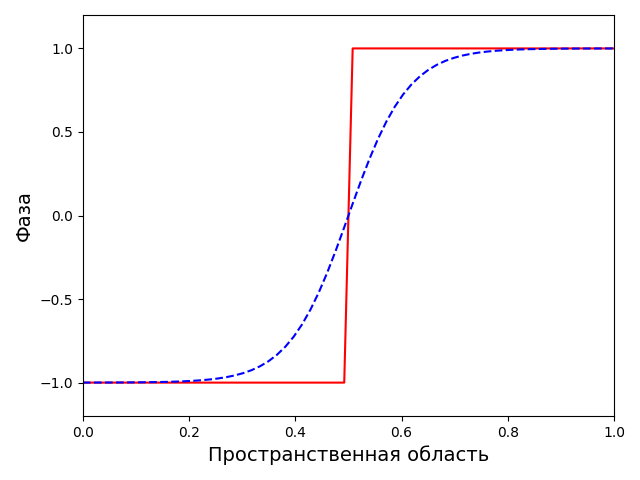
\includegraphics[width=\linewidth]{images/data0.png}
        \subcaption{Фаза при \( t = 0 \): начальное распределение. Сплошная линия~--- численное решение, пунктирная~--- аналитическое решение}
        \label{fig:modeling_KH:1}
    \end{minipage}
    \hfill
    \begin{minipage}{0.49\linewidth}
        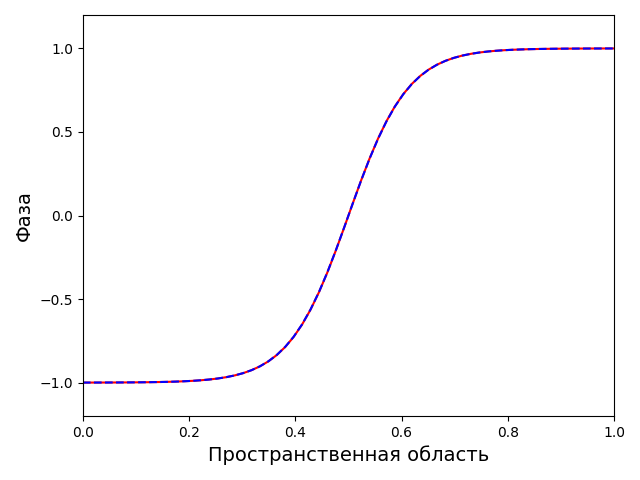
\includegraphics[width=\linewidth]{images/data40000000.png}
        \subcaption{Фаза при \( t = 0.12 \). Сплошная линия~--- численное решение, пунктирная~--- аналитическое решение}
        \label{fig:modeling_KH:2}
    \end{minipage}
    
    % Second Row
    \begin{minipage}{0.49\linewidth}
        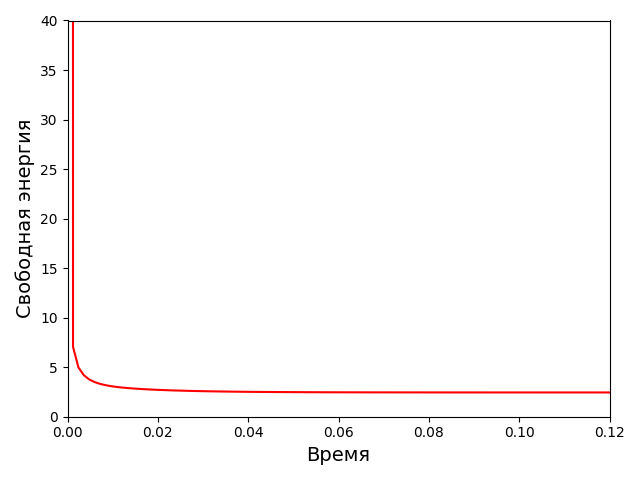
\includegraphics[width=\linewidth]{images/data_energ.png}
        \subcaption{Динамика свободной энергии системы в зависимости от времени \( t \)}
        \label{fig:modeling_KH:3}
    \end{minipage}
    \hfill
    \begin{minipage}{0.49\linewidth}
        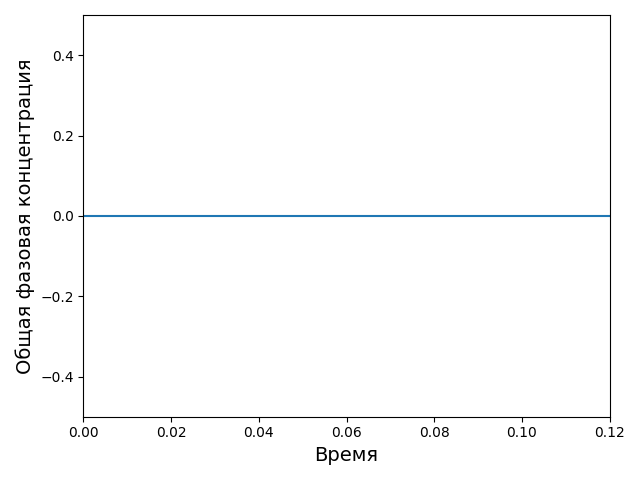
\includegraphics[width=\linewidth]{images/phase_balance.png}
        \subcaption{Сохранение общей концентрации фазы в течении времени \( t \)}
        \label{fig:modeling_KH:4}
    \end{minipage}
    
    \caption{Моделирование уравнения Кана-Хилларда: точное решение и результаты моделирования для различных временных моментов.}
    \label{fig:modeling_KH}
\end{figure}

В экспериментах обычно наблюдается разделение бинарной среды на домены с профилем перехода, который описывается уравнением~(\ref{analit}). Величина $\sqrt{\beta}$ определяет типичную ширину переходного слоя между доменами.
Поскольку для $\phi$ выполняется уравнение непрерывности~(\ref{neprerivn}), в процессе эволюции сохраняется общая концентрация фазы:
\begin{equation*}
    C = \int \limits_{\Omega} \phi(x, t) \, dx, \quad \frac{dC}{dt} = 0.
\end{equation*}
В качестве начального условия моделирования используем две несмешанные фазы, описываемые фазовой функцией:
\begin{equation*}
    \phi(x) = -1.0 + 2.0 \cdot H(x - x_0),
\end{equation*}
где $H(x)$~--- функция Хевисайда.

Для моделирования будем использовать следующие параметры: размер области $L = 1.0$, шаг сетки: $ h = 1 / 64$, временной шаг $\Delta t = h^4 / 20$, параметр $\beta = 25h^2$; подвижность $K = 1$.

Граничные условия задаются как:
\begin{equation*}
\phi(0) = -\phi(L) = -1.0, \nabla^2\phi(0) = \nabla^2\phi(L) = 0.
\end{equation*}

Моделирование показывает, что переходный слой стремится к аналитическому решению~(\ref{analit}) уравнения Кана-Хиларда.
Для подтверждения сохранения концентрации фазы, изобразим динамику баланса фазы во времени на рисунке~\ref{fig:modeling_KH:3}. Кроме того, визуализируем изменение свободной энергии~(\ref{energ}) системы с течением времени на рисунке~\ref{fig:modeling_KH:4}.


\subsection{Одномерный кристалл}
%Одномерный кристалл------------------------------------------------------------
Произведём моделирование кристаллической структуры, эволюция которой описывается уравнением~(\ref{evolution_eq}). В этой модели фазовое поле интерпретируется как атомная плотность.
Зафиксируем параметры уравнения~(\ref{delta psi}) следующим образом: $\beta = -2$, $\gamma = 1$, $\epsilon = 1$, $K = 1$.

Получаем следующее уравнение эволюции:
\begin{equation*}
    \frac{\partial \phi}{\partial t} = \operatorname{div}\left[\operatorname{grad} \left(
    \alpha \phi + 2 \Delta \phi + \Delta^2 \phi +
    \phi^3 - \phi\right)\right].
\end{equation*}

Сделав замену $r = \alpha -2$, приведем это уравнение к виду:

\begin{equation*}
    \frac{\partial \phi}{\partial t} = \frac{\partial \phi}{\partial t} = \Delta\left[
    (1 + \Delta)^2 \phi + \phi^3 + r \phi\right].
\end{equation*}

\label{parametrs1}
Остальные параметры для моделирования положим следующим образом: размер области $L = 40.0$, шаг сетки $\displaystyle h = 0.4$, временной шаг $\displaystyle \Delta t = 10^{-4}$, параметр $r = -0.4$.

Начальное условие выберем как случайное возмущение вблизи нуля со средним значением равным 0, а за граничные условия возьмём периодические граничные условия.

Результаты моделирования показаны на рисунках~\ref{fig:modeling_1_d}. На рисунке~\ref{fig:modeling_1_d:1} показано начальное условие, на рисунках~\ref{fig:modeling_1_d:2}-\ref{fig:modeling_1_d:4}~--- распределение фазового поля в моменты времени $t = 1, 10, 100$. Как видно из полученных графиков, фаза в процессе эволюции принимает вид периодической функции, а свободная энергия монотонно и резко убывает.

\begin{figure}[p]
    \centering
    % First Row
    \begin{minipage}{0.49\linewidth}
        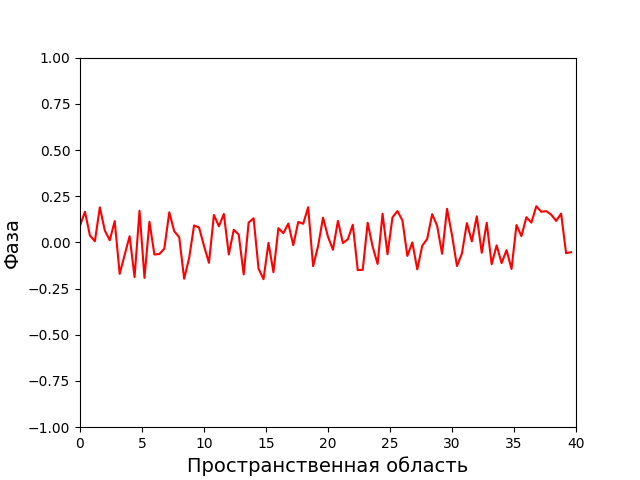
\includegraphics[width=\linewidth]{images/3-data_data_0.bin.png}
        \subcaption{Поле атомной плотности при \( t = 0 \): начальное распределение}
        \label{fig:modeling_1_d:1}
    \end{minipage}
    \hfill
    \begin{minipage}{0.49\linewidth}
        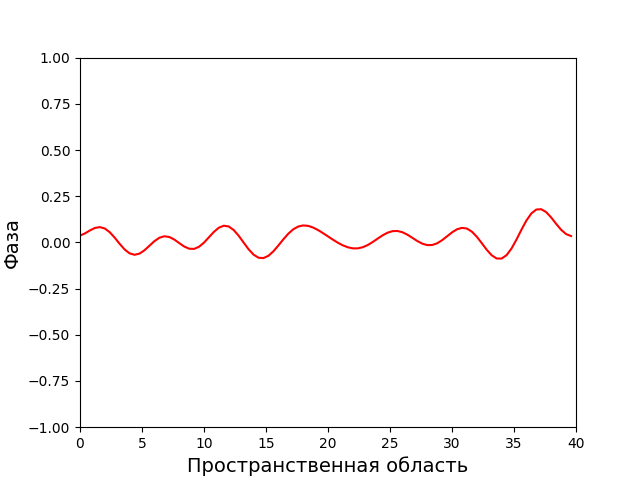
\includegraphics[width=\linewidth]{images/3-data_data_10000.bin.png}
        \subcaption{Поле атомной плотности при \( t = 1 \)}
        \label{fig:modeling_1_d:2}
    \end{minipage}

    % Second Row
    \begin{minipage}{0.49\linewidth}
        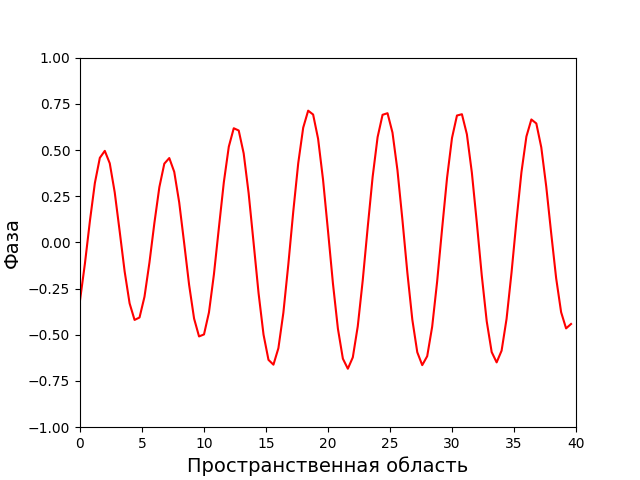
\includegraphics[width=\linewidth]{images/3-data_data_100000.bin.png}
        \subcaption{Поле атомной плотности при \( t = 10 \)}
        \label{fig:modeling_1_d:3}
    \end{minipage}
    \hfill
    \begin{minipage}{0.49\linewidth}
        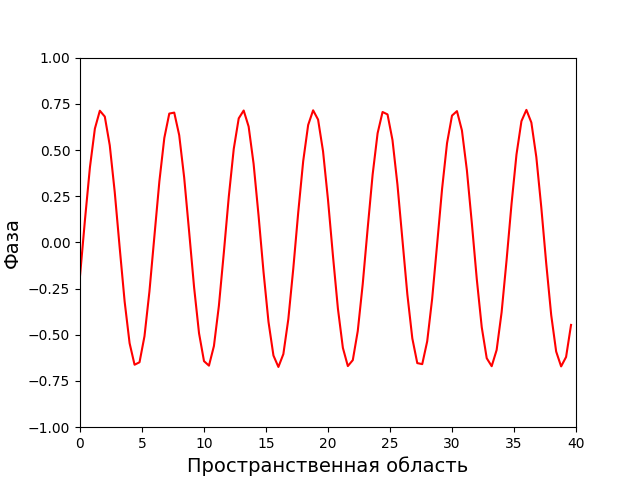
\includegraphics[width=\linewidth]{images/3-data_data_1000000.bin.png}
        \subcaption{Поле атомной плотности при \( t = 100 \)}
        \label{fig:modeling_1_d:4}
    \end{minipage}
    
    % Third Row
    \begin{minipage}{0.49\linewidth}
        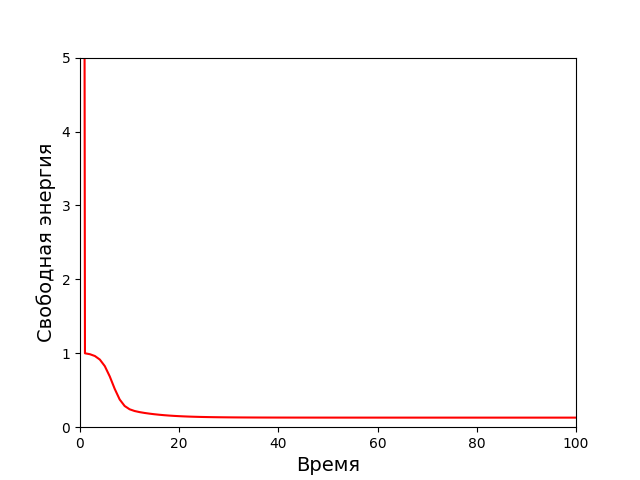
\includegraphics[width=\linewidth]{images/3-energy.png}
        \subcaption{Динамика свободной энергии системы в зависимости от времени \( t \)}
        \label{fig:modeling_1_d:5}
    \end{minipage}
    \hfill
    \begin{minipage}{0.49\linewidth}
        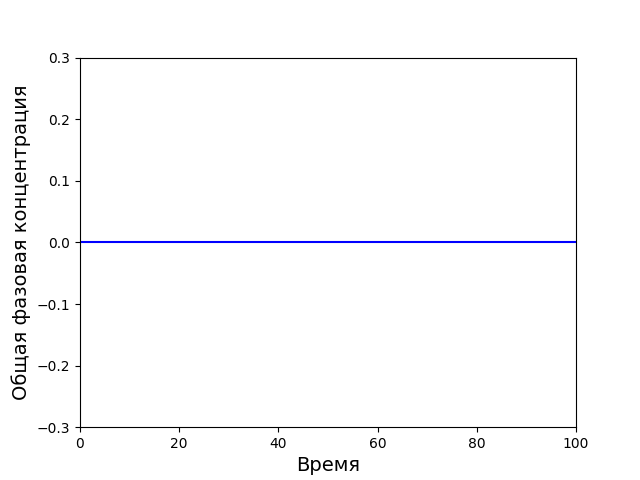
\includegraphics[width=\linewidth]{images/3-phase_balance.png}
        \subcaption{Сохранение общей концентрации фазы в течении времени \( t \)}
        \label{fig:modeling_1_d:6}
    \end{minipage}
    
    \caption{Моделирование одномерной кристаллической структуры}
    \label{fig:modeling_1_d}
\end{figure}


\begin{figure}[p]
    \centering
    % First Row
    \begin{minipage}{0.49\linewidth}
        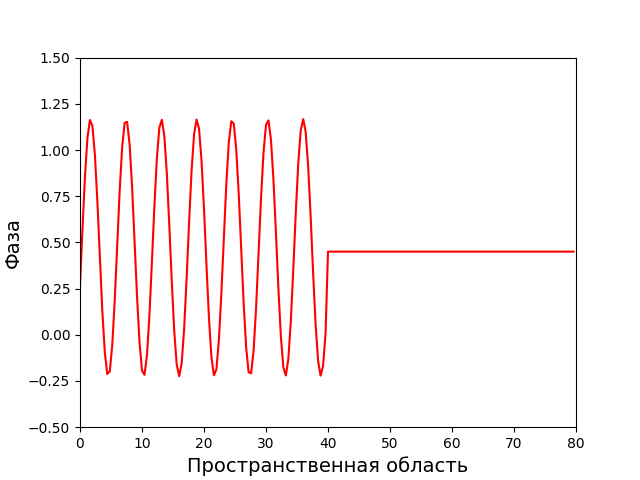
\includegraphics[width=\linewidth]{images/4-data_data_0.bin.png}
        \subcaption{Начальное условие с $\phi_0 = 0.45$}
    \end{minipage}
    \hfill
    \begin{minipage}{0.49\linewidth}
        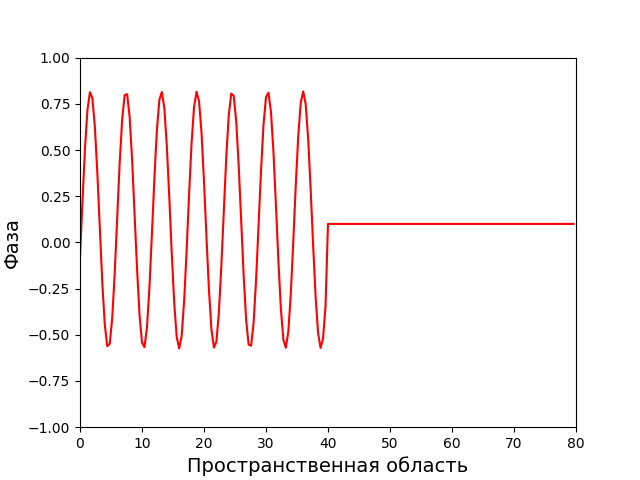
\includegraphics[width=\linewidth]{images/5-data_data_0.bin.png}
        \subcaption{Начальное условие с $\phi_0 = 0.1$}
    \end{minipage}
    \caption{Начальные условия соответствующие двум случаям}
    \label{fig:begin_equation}

    \centering
    % First Row
    \begin{minipage}{0.49\linewidth}
        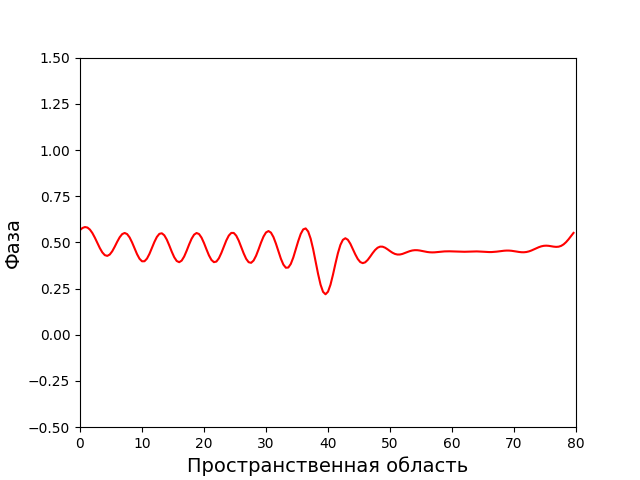
\includegraphics[width=\linewidth]{images/4-data_data_50000.bin.png}
        \subcaption{Фазовое поле при \( t = 5 \)}
    \end{minipage}
    \hfill
    \begin{minipage}{0.49\linewidth}
        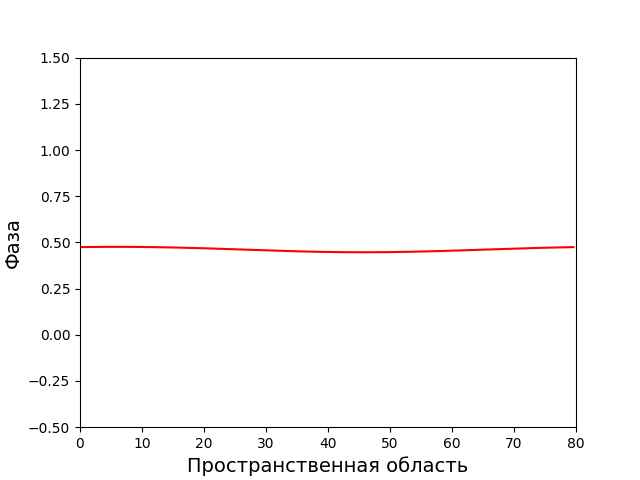
\includegraphics[width=\linewidth]{images/4-data_data_1000000.bin.png}
        \subcaption{Фазовое поле при \( t = 100 \)}
    \end{minipage}
    \caption{Эволюция фазовой функции в первом случае}
    \label{fig:evolution_1}

    \centering
    % First Row
    \begin{minipage}{0.49\linewidth}
        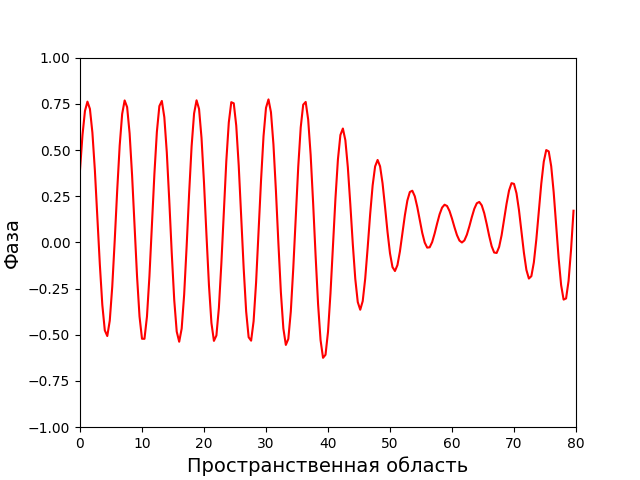
\includegraphics[width=\linewidth]{images/5-data_data_50000.bin.png}
        \subcaption{Фазовое поле при \( t = 5 \)}
    \end{minipage}
    \hfill
    \begin{minipage}{0.49\linewidth}
        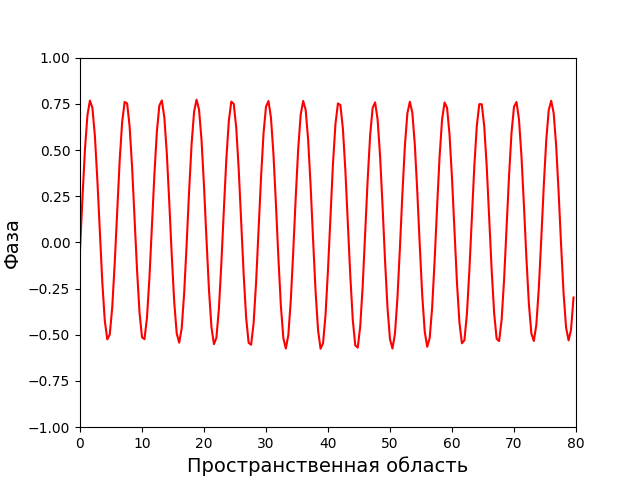
\includegraphics[width=\linewidth]{images/5-data_data_1000000.bin.png}
        \subcaption{Фазовое поле при \( t = 100 \)}
    \end{minipage}
    \caption{Эволюция фазовой функции во втором случае}
    \label{fig:evolution_2}
\end{figure}

\subsection{Зависимость амплитуды фазового поля\\от параметров}
Параметр $r$ играет роль температуры. 
\begin{equation*}
    r \sim \frac{T - T_c}{T_c},
\end{equation*}
где $T_c$~--- температура кристаллизации.

В статье Элдера и Гранта~\cite{elder_2004} анализируется зависимость амплитуды фазовой функции, получающейся в процессе эволюции, от параметра $r$ и начального распределения фазы. Приводится следующее выражение:
\begin{equation*}
    A = 2 \sqrt{- r / 3 - \phi_0^2},
\end{equation*}
где $A$~--- амплитуда фазовой функции, а $\phi_0$~--- среднее значение фазы.
В случае отрицательного значения выражения под корнем, фаза в процессе эволюции стремится к константе, что соответствует распределению фазы в жидкости.

Таким образом, даже при температуре меньшей температуры кристаллизации и отрицательном параметре $r$ кристаллизации может не происходить по причине достаточно большой средней фазовой концентрации $\phi_0$.

Смоделируем два случая соответствующие разным знакам выражения под корнем за счёт изменения среднего значения фазы. Моделирование будем проводить на области размером $2 L = 80.0$, a начальное условие будем задавать в виде:
\[
\phi(x) = 
\left\{
\begin{array}{ll}
    \phi_0 + \phi^*(x), & 0 \leqslant x < L,\\
    \phi_0, & L \leqslant x < 2 L,
\end{array}
\right.
\]
где $\phi^*(x)$~--- фазовая функция получаемая в результате моделирования с параметрами из раздела~(\ref{parametrs1}). Среднее значение будет принимать значения $0.45$ в первом случае и $0.1$ во втором. Остальные параметры положим как в разделе~(\ref{parametrs1}).

На рисунках~\ref{fig:begin_equation} приведены графики начального распределения фазы в обоих случаях, отличающихся друг от друга средним значением фазы. Они могут быть интерпретированы как кристалл помещённый в жидкость при температуре и фазовой концентрации соответствующих плавлению кристалла в первом случае и кристаллизации жидкости во втором.

Рисунки~\ref{fig:evolution_1} соответствуют эволюции фазовой функции в случае большего значения фазы. В процессе эволюции наблюдается плавление кристалла. Получаемое в результате $100$ секунд эволюции распределение близко к константе и имеет физический смысл распределения атомной плотности в жидкости.

Рисунки~\ref{fig:evolution_2} соответствуют эволюции фазовой функции в случае меньшего среднего значения фазы. В процессе эволюции наблюдается кристаллизация жидкости. Получаемое в результате $100$ секунд эволюции распределение отлично от константы и имеет периодическую структуру. Физический смысл получающегося распределения фазы~--- атомная плотность в кристалле.

